\section{A New Program for Graph Representation Learning}\label{sec: new challenges}


\begin{figure}[h] % 'h' for here
  \centering
  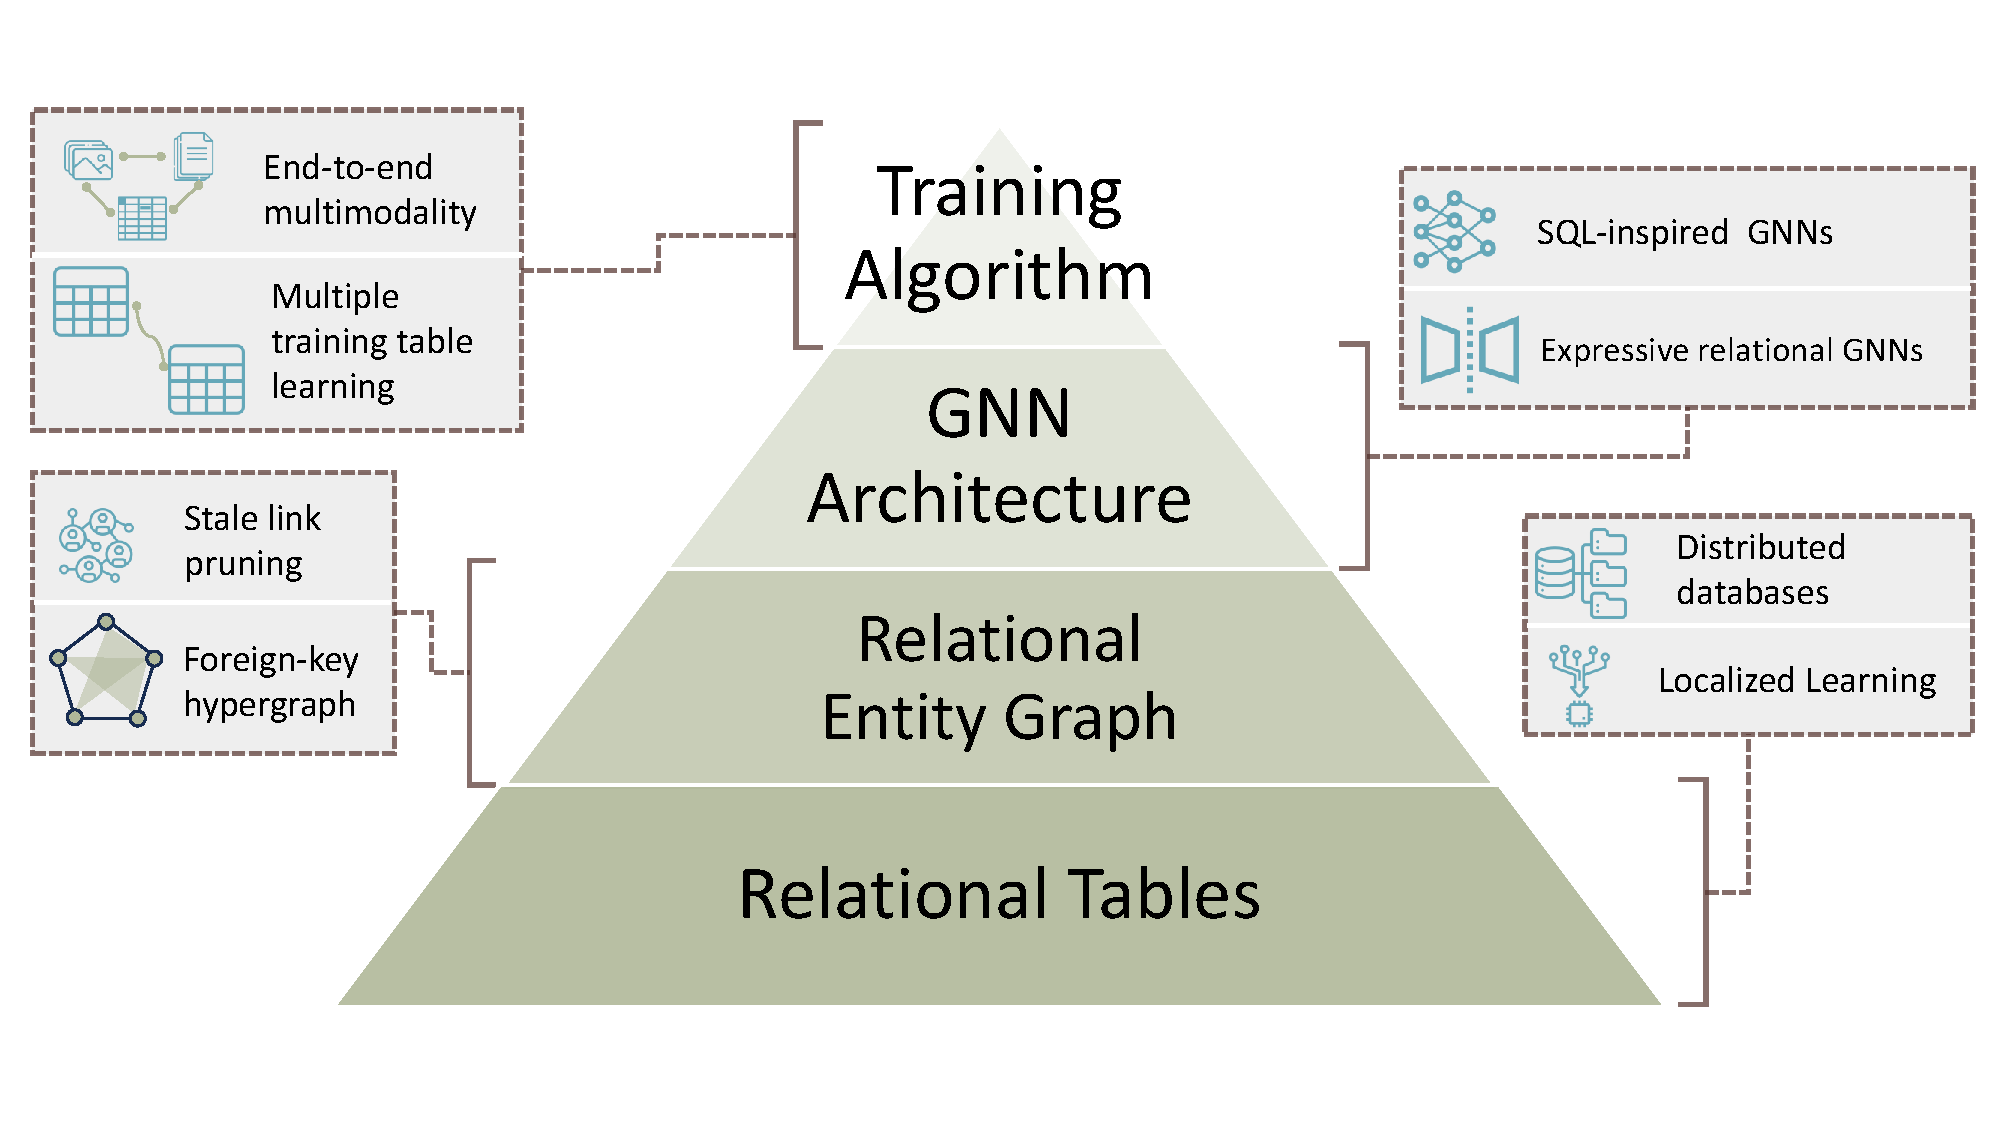
\includegraphics[width=0.9\linewidth]{figs/landscape.pdf}
  \caption{\AreaName brings new challenges at all levels of the machine learning stack.}
  \label{fig: research landscape}
\end{figure}

Developing \AreaName requires a new research program in graph representation learning on relational data. There are opportunities at all levels of the research stack, including (pre-)training methods, GNN architectures, multimodality, new graph formulations, and scaling to large distributed relational databases for many industrial settings. Here we discuss several promising aspects of this research program, aiming to stimulate the interest of the graph machine learning community.


\subsection{Scaling \AreaName}

Relational databases are often vast, with information distributed across many servers with constrained communication. However, relational data has a non-typical graph structure which may help scale \AreaName more efficiently.


\xhdr{Distributed Training on Relational Data} Existing distributed machine learning techniques often assume that each server contains data of the same type. Relational data on the other hand, naturally partitions in to pieces, bringing new challenges depending on the partitioning technique used. \emph{Horizontal partitioning}, known as sharding, is the most common approach. It creates database shards by splitting tables row-wise according to some criterion (e.g., all customer with zipcode in a given range). In this case, a table containing a customers personal record may lie on a distinct server from the table recording recent purchase activity, leading to communication bottlenecks when attempting to train models by sensing messages between purchases and customer records. Less common, but also possible, is vertical splitting. Different splitting options suggests an opportunity to (a) develop specialized distributed learning methods that exploit the vertical or horizontal partitioning, and (b) design further storage arrangements that may be more suited to \AreaName. The question of graph partitioning arises in all large-scale graph machine learning settings, however in this case we are fortunate to have non-typical graph structure (i.e., it follows the schema) which makes it easier to find favourable partitions.

\xhdr{Localized Learning} For many predictive tasks it is neither feasible (due to database size) nor desirable (due to task narrowness) to propagate GNN messages across the entire graph during training. In such cases, sampling schemes that preserve locality by avoiding exponential growth in GNN receptive field are needed. This is easily addressed in cases with  prior knowledge on the relevant entities. How to scale to deep models that remain biased models towards local computation in cases with no prior knowledge remains an interesting open question.



\subsection{Building Graphs from Relational Data}

An essential ingredient of \AreaName is the use of an individual entity and relation-level graph on which to apply inter-entity message passing to learn entity embeddings based on relations to other entities.  In Sec. \ref{sec:formal_rl_graph} we introduced one such graph, the \emph{relational entity graph}, a general procedure for viewing any relational database as a graph. Whilst a natural choice, we do not propose dogmatically viewing entities as nodes and relations as edges.  Instead, the essential property of the relational entity graph is that it is \emph{full-resolution}. That is, each entity and each primary-foreign key link in the relational database corresponds to its own graph-piece, so that the relational database is exactly encoded in graph form. It is this property that we expect potential alternative graph designs to share. Beyond this stipulation, many creative graph choices are possible, and we discuss some possibilities here.


\xhdr{Foreign-key Hypergraph} Fact tables often contain entities with a fixed foreign-key pattern (\emph{e.g.}, in \Amazon a row in a \tbl{review} table always refers to a \tbl{customer} and a \tbl{product} foreign key). The relational entity graph views a review as a node, with edges to a customer and product. However, another possibility is to view this as a single hyperedge between review, customer, and product. Alternative graph choices may alter (and improve) information propagation between entities (\emph{cf.} Sec. \ref{sec: new gnns}). 


\xhdr{Stale Link Pruning} Entities that have been active for a long time may have a lot of links to other entities. Many of these links may be \emph{stale}, or uninformative, for certain tasks. For example, the purchasing patterns of a longtime customer during childhood are likely to be less relevant to their purchasing patterns in adulthood. Links that are stale for a certain task may hurt predictive power by obfuscating true predictive signals, and reduce model efficiency due to processing uninformative data. This situation calls for careful stale link and entity handling to focus on relevant information. Promising methods may include pruning or preaggregating stale links. More generally, how to deal with more gradual distribution drift over time is an open question. 


\subsection{GNN Architectures for Relational Data}\label{sec: new gnns}

Viewing a relational database a graphs leads to graphs with structural properties that are consistent across databases. To properly exploit this structure new specialized GNN architectures are needed. Here we discuss several concrete directions for designing new architectures.

\xhdr{Expressive GNNs for Relational Data} Relational entity graphs (\emph{cf.} Sec. \ref{sec:formal_rl_graph}) obey certain structural constraints. For example, as nodes correspond to entities drawn from one of several tables, the relational entity graph is naturally $n$-partite, where $n$ is the total number of tables.  This suggests that GNNs for relational data should be designed to be capable of learning expressive decision rules over $n$-partite graphs. Unfortunately,  recent studies find that many GNN architectures fail to distinguish biconnected graphs \citep{zhang2023rethinking}. Further work is needed to design expressive $n$-partite graph models.

Relational entity graphs also have regularity in edge-connectivity. For instance, in \Amazon entities in the \tbl{review} table always refer to one \tbl{customer} and one \tbl{product}.
Consistent edge patterns are described by the structure of the schema graph $(\mathcal T, \mathcal R)$ (\emph{cf.} Sec. \ref{sec:schema_graph}). How to integrate prior knowledge of the graph structure of $(\mathcal T, \mathcal R)$ into GNNs that operate on an entity-level graph (the relational entity graph) remains an open question. These two examples serve only to illustrate the possibilities for architecture design based on the structure of relational entity graphs. Many other structural properties of relational data may lead to innovative new expressive GNN architectures.


\xhdr{Query Language Inspired Models} SQL operations are known to be extremely powerful operations for manipulating relational data. Their weakness is that they do not have differentiable parameters, making end-to-end learnability impossible. Despite this, there are close similarities between key SQL queries and the computation process of graph neural networks. For instance, a very common way to combine information across tables $T_1,T_2$ in SQL is to (1) create a table $T_3$ by applying a \texttt{JOIN} operation to table $T_1$ and $T_2$, by matching foreign keys in $T_1$ to primary keys in $T_2$, then (2) produce a final table with the same number of rows as $T_2$ by applying an \texttt{AGGREGATE} operation to rows in $T_3$ with foreign keys pointing to the same entity in $T_2$. There are many choices of \texttt{AGGREGATE} operation such as \texttt{SUM}, \texttt{MEAN}  and  \texttt{COUNT}. This process \emph{directly} mirrors GNN computations of messages from neighboring nodes, followed by message aggregation. In other words, GNNs can be thought of as a neural version of SQL \texttt{JOIN}+\texttt{AGGREGATE} operations. This suggests that an opportunity for powerful new neural network architectures by designing differentiable computation blocks that algorithmically align \citep{xu2019can} to existing SQL operations that are known to be useful.


\xhdr{New Message Passing Schemes} Beyond expressivity, new architectures may also improve information propagation between entities. For instance, collaborative filtering methods enhance predictions by identify entities with similar behavior patterns, customers with similar purchase history. However, in the relational entity graph, the two related customers may not be directly linked. Instead they are indirectly be linked to one another through links to their respective purchases, which are linked to a particular shared product ID. This means that a standard message passing GNN will require four message passing steps to propagate the information that customer $v_1$ purchased the same product as customer $v_2$ (2-hops from $v_1$ to product, and 2-hops from product to $v_1$). New message passing schemes that do multiple hops or directly connect customers (more generally, entities) with similar behavior patterns may more effectively propagate key information through the model. As well as new message passing schemes, there is also opportunity for new message aggregation methods. One possibility is order dependent aggregation, that combines messages in a time-dependent way, as explored by \cite{yang2022stam}. Another is schema dependent aggregation, that combines messages based on what part of the schema graph the messages are arriving from.


\subsection{Training Techniques for Relational Data}

By its nature, relational data contains highly overlapping predictive signals and tasks. This interconnectedness of data and tasks is a big opportunity for new neural network training methods that maximally take advantage of this interconnectedness to identify useful predictive signals. This section discusses several such opportunities.


\xhdr{Multi-Task Learning} 
 Many predictive tasks on relational data are distinct but related. For example, predicting customer lifetime value, and forecasting individual product sales both involve anticipating future purchase patterns. In {\BenchmarkName}, this corresponds to defining multiple training tables, one for each task, and training a single model jointly on all tasks in order to benefit from shared predictive signals. How to group training tables to leverage their overlap is a promising area for further study. 


\xhdr{Multi-Modal Learning}

Entities in relational databases often have attributes covering multiple modalities (\emph{e.g.,} products come with images, descriptions, as well as different categorical and numerical features). The \AreaName blueprint first extracting entity-level features, which are used as initial node-features for the GNN model.
In \BenchmarkName, this multimodal entity-level feature extraction is handled by using state-of-the-art pre-trained models using the PyTorch Frame library to pre-extract features. This maximizes convenience for graph-focused research, but is likely suboptimal because the entity-level feature extraction model is frozen. This is especially relevant in contexts with unusual data---e.g., specialized medical documentation---that generic pre-trained models will likely fail to extract important details.
To facilitate exploration of joint entity-level and graph-level modelling, \BenchmarkName also provides the option to load raw data, to allow researchers to experiment with different feature-extraction methods.

\xhdr{Foundation Models and Data Type Encoders} In practice, new predictive tasks on relational data are often specified on-the-fly, with fast responses required. Such situations preclude costly model training from scratch, instead requiring powerful and generic pre-trained models. Self-supervised labels for model pre-training can be mined from historical data, just as with training table construction. However, techniques for automatically deciding which labels to mine remains unexplored. Another desirable property of pre-trained models is that they are \emph{inductive}, so they can be applied to entirely new relational databases out-of-the-box. This presents a challenges in how to deal with unseen column types and relations between tables. Such flexibility is needed in order to move towards foundation models for relational databases. More broadly, how to build column encoders is an important question. As well as distribution shifts as mentioned in the previous paragraph, there are also decisions on when to share column encoders (should two image columns use the same image encoder?), as well as special data types such as static time intervals (\emph{e.g.}, to describe the time period an employee worked at a company, or the time period in which a building project was conducted). Special data types may require specialized encoder choices, and possibly even deeper integration into the neural network computation graph. How best to aggregate of cross-modal information into a single fused embedding is another question for exploration. 

